%%%%%%%%%%%%%%%%%%%%%%%%%%%%%%%%%%%%%%%%%%%%%%%%%%%%%%%%%%%%%%%%%%%%%%%%%%%

\documentclass[a4paper,oneside,12pt]{article}
\usepackage{mystyle}

\begin{document}

\title{\Large\bf Applications of quadratic functions}
\author{%%
  Minh Van Nguyen \\
  \url{mvngu@gmx.com}
}
\date{\today}
\maketitle


\begin{packeditem}
\item Application: gravity and displacement of projectile.

\item Area under a quadratic function.
\end{packeditem}

This document will show you how the quadratic function can be used in
a variety of situations.  The document consists of mostly worked
examples and exercises.


%%%%%%%%%%%%%%%%%%%%%%%%%%%%%%%%%%%%%%%%%%%%%%%%%%%%%%%%%%%%%%%%%%%%%%%%%%%

\section{Geometry}

\begin{example}
\textbf{Fencing.}
\label{ex:fence_a_rectangular_region}
You want to install a fence around a rectangular region that has an
area of $7$ metres squared.  You want the length of the rectangular
region to be two metres longer than the width.  Calculate the width of
the region.
\end{example}

\begin{solution}
Whenever possible, you should first draw a picture to help you solve a
problem.  In this example, the rectangular region and its dimensions
can be illustrated as shown in
\Figure{fig:rectangular_region_7_metres_squared}.  Since the width of
the region is $w$ metres and its length is $w + 2$ metres, the area of
the region is $(w + 2)w$ metres squared.  However, you also know that
the region has an area of $7$~metres squared, which can be used to
give you the equation
%%
\begin{equation}
\label{eqn:rectangular_region_equation}
(w + 2)w
=
7.
\end{equation}

\begin{figure}[!htbp]
\centering
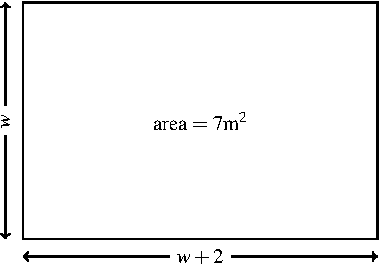
\includegraphics[scale=1]{image/09/rectangular-fence.pdf}
\caption{%%
  A rectangular region whose area is $7$ metres squared.  The width of
  the region is denoted $w$.
}
\label{fig:rectangular_region_7_metres_squared}
\end{figure}

Let's determine all values of $w$ that satisfy
\Equation{eqn:rectangular_region_equation}.  Expand the left-hand side
of \Equation{eqn:rectangular_region_equation} to get $w^2 + 2w = 7$.
Upon moving everything to the left-hand side, you end up with the
quadratic equation
%%
\begin{equation}
\label{eqn:rectangular_region_quadratic}
w^2 + 2w - 7
=
0.
\end{equation}
%%
Writing the left-hand side as $f(w) = w^2 + 2w - 7$,
\Equation{eqn:rectangular_region_quadratic} can also be written as
$f(w) = 0$.  This means that you want to determine all roots of
$f(w)$.  Before calculating the roots of $f(w)$, you investigate
whether $f(w)$ has a unique root, two different roots, or the graph of
$f(w)$ does not intersect the horizontal axis.  This is a job for the
discriminant.  The discriminant of $f(w)$ is $\Delta = 32$.  This is a
positive number so there exists at least one real value of $w$ that
solves \Equation{eqn:rectangular_region_equation}.  Using the
quadratic formula, the roots of $f(w)$ can be written as
$w = -1 \pm 2\sqrt{2}$.  One root of $f(w)$ is given by
\[
w_1
=
2\sqrt{2} - 1
\]
which is positive.  The other root is given by
\[
w_2
=
-2\sqrt{2} - 1
\]
which is negative.  You reject the number $w_2$ because the width of
the rectangular region cannot be a negative number.  To confirm your
decision to reject the root $w_2$, you sketch a graph of $f(w)$ as
shown in \Figure{fig:rectangular_region_quadratic_roots} and note that
$w_2$ is located on the negative half of the $w$-axis, i.e.~the
horizontal axis.  You conclude that the width of the rectangular
region is approximately $2\sqrt{2} - 1 \approx 1.8284$ metres long,
rounded to four decimal places.
\end{solution}

\begin{figure}[!htbp]
\centering
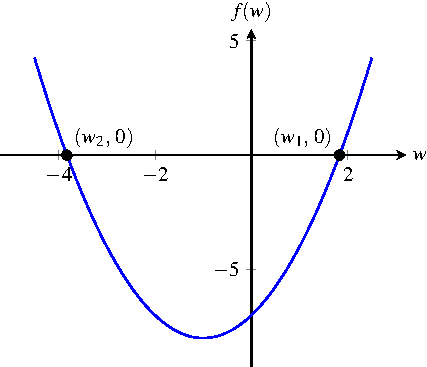
\includegraphics[scale=1]{image/09/a1-b2-cminus7.pdf}
\caption{%%
  Graph of the function $f(w) = w^2 + 2w - 7$.  The two dots indicate
  the two different roots of $f(w)$.
}
\label{fig:rectangular_region_quadratic_roots}
\end{figure}

\begin{exercise}
\label{ex:rectangular_region_discriminant}
In the solution of \Example{ex:fence_a_rectangular_region}, verify
that the discriminant is $\Delta = 32$.
\end{exercise}
%%
\ifbool{showSolution}{
\begin{solution}
In the equation $f(w) = w^2 + 2w - 7$, you have the values $a = 1$,
$b = 2$, and $c = -7$.  Use \Definition{def:discriminant} to see that
the discriminant of $f(w)$ is
%%
\begin{align*}
\Delta
&=
2^2 - 4(1)(-7) \\[4pt]
&=
4 + 28 \\[4pt]
&=
32
\end{align*}
%%
as required.
\end{solution}
}{}

\begin{exercise}
In the solution of \Example{ex:fence_a_rectangular_region}, verify
that the roots of $f(w)$ can be written as $w = -1 \pm 2\sqrt{2}$.
\end{exercise}
%%
\ifbool{showSolution}{
\begin{solution}
You have the equation $f(w) = w^2 + 2w - 7$, whose roots can be
calculated by using the quadratic formula.  The discriminant of $f(w)$
is known to be $\Delta = 32$, as verified in
\Exercise{ex:rectangular_region_discriminant}, so the roots are
%%
\begin{align*}
w
&=
\frac{
  -2 \pm \sqrt{\Delta}
}{
  2(1)
} \\[4pt]
&=
\frac{
  -2 \pm \sqrt{2 \times 4^2}
}{
  2
} \\[4pt]
&=
\frac{
  -2 \pm 4\sqrt{2}
}{
  2
} \\[4pt]
&=
\frac{
  2(-1 \pm 2\sqrt{2})
}{
  2
} \\[4pt]
&=
-1 \pm 2\sqrt{2}
\end{align*}
%%
as required.
\end{solution}
}{}

\begin{example}
\label{ex:running_ants}
\textbf{Ant race.}
Two ants are next to each other.  Ant $A$ runs eastward at a rate of
two centimetres per second.  After one second since ant $A$ started
running, ant $B$ runs northward also at the same rate.  How long since
ant $A$ started running does it take for both ants to be five
centimetres apart?
\end{example}

\begin{solution}
As in \Example{ex:fence_a_rectangular_region}, you should first draw a
picture that can help you in solving the problem.  Denote by $t$ the
time in seconds and use $t$ to represent the amount of time that ant
$A$ runs.  Since ant $A$ runs in the eastern direction at two
centimetres per second, after $t$ seconds the ant would have covered a
horizontal distance of $2t$ centimetres.  When ant $A$ starts running,
ant $B$ is still at the starting position and must wait one second
before it starts to run in the northern direction.  The amount of time
that ant $B$ runs is one second less than the amount of time that ant
$A$ runs.  In other words, the duration of time that ant $B$ runs can
be written as $t - 1$ seconds, after which the ant would have
travelled a vertical distance of $2(t - 1)$ centimetres.  The
situation is illustrated in \Figure{fig:running_ants_triangle}.

\begin{figure}[!htbp]
\centering
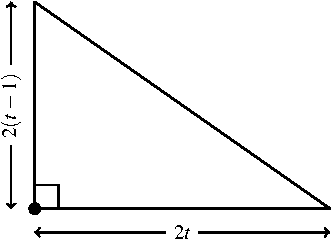
\includegraphics[scale=1]{image/09/running-ants.pdf}
\caption{%%
  A right-angled triangle that represents the directions in which two
  ants run.  The dot indicates the starting position of the ants.  The
  variable $t$ denotes time in seconds.  After $t$ seconds, the
  distance between the ants is represented by the length of the
  hypotenuse.
}
\label{fig:running_ants_triangle}
\end{figure}

Let's now formulate the problem as an equation.  The horizontal and
vertical distances travelled by both ants can be represented as the
base and height, respectively, of the right-angled triangle in
\Figure{fig:running_ants_triangle}.  After $t$ seconds have passed,
the distance between the ants is represented by the length of the
hypotenuse of the triangle.  Using Pythagoras' theorem, the problem
can be formulated as the quadratic equation
%%
\begin{equation}
\label{eqn:running_ants_quadratic_equation}
8t^2 - 8t + 4
=
25.
\end{equation}

The problem now is to determine all values of $t$ that satisfy
\Equation{eqn:running_ants_quadratic_equation}.  Note that the
equation can also be written as
\[
8t^2 - 8t - 21
=
0.
\]
Writing $f(t) = 8t^2 - 8t - 21$,
\Equation{eqn:running_ants_quadratic_equation} is equivalent to the
equation $f(t) = 0$, hence the values of $t$ that satisfy
\Equation{eqn:running_ants_quadratic_equation} are the same as the
roots of $f(t)$.  The quadratic formula shows that the roots of $f(t)$
are
%%
\begin{equation}
\label{eqn:running_ants_roots}
t_1
=
\frac{1}{2}
+
\frac{\sqrt{46}}{4}
%%
\qquad
\text{and}
\qquad
%%
t_2
=
\frac{1}{2}
-
\frac{\sqrt{46}}{4}.
\end{equation}
%%
You reject the root $t_2$ because it is negative.  A negative value of
time does not make sense in the context of the problem.  Therefore the
ants would be five centimetres apart after approximately
$\frac{1}{2}
+
\frac{\sqrt{46}}{4}
\approx
2.1956$
seconds~(rounded to four decimal places) since ant $A$ started running.
\end{solution}

\begin{exercise}
Explain why \Example{ex:running_ants} can be represented as
\Equation{eqn:running_ants_quadratic_equation}.
\end{exercise}
%%
\ifbool{showSolution}{
\begin{solution}
From \Figure{fig:running_ants_triangle} you know that after $t$
seconds, ant $A$ would have travelled $2t$ centimetres and ant $B$
would have travelled $2(t - 1)$ centimetres.  These numbers are the
base and height, respectively, of a right-angled triangle.  After $t$
seconds, the distance between the ants is represented by the  length
of the hypotenuse in \Figure{fig:running_ants_triangle}.  You want to
know when the ants are $5$ centimetres apart, so the hypotenuse is $5$
centimetres.  By Pythagoras' theorem, the three sides of the
right-angled triangle are related by the equation
\[
(2t)^2 + \bigparen{2 (t - 1)}^2
=
5^2.
\]
Upon expanding the parentheses, the equation can be written as
\[
4t^2 + (2t - 2)^2
=
25.
\]
Expand the remaining pair of parentheses to get
\[
4t^2 + 4t^2 - 8t + 4
=
25.
\]
After collecting like terms, you end up with
\Equation{eqn:running_ants_quadratic_equation}.
\end{solution}
}{}

\begin{exercise}
In the solution to \Example{ex:running_ants}, verify that the roots of
$f(t)$ are those given by~\eqref{eqn:running_ants_roots}.
\end{exercise}
%%
\ifbool{showSolution}{
\begin{solution}
You have the quadratic function $f(t) = 8t^2 - 8t - 21$.  Using the
quadratic formula, the roots of $f(t)$ are
%%
\begin{align*}
t
&=
\frac{
  -(-8) \pm \sqrt{(-8)^2 - 4(8)(-21)}
}{
  2(8)
} \\[4pt]
&=
\frac{
  8 \pm \sqrt{736}
}{
  16
} \\[4pt]
&=
\frac{
  8 \pm \sqrt{4^2 \times 2 \times 23}
}{
  16
} \\[4pt]
&=
\frac{
  8 \pm 4\sqrt{46}
}{
  16
} \\[4pt]
&=
\frac{
  4 \parenthesis*{2 \pm \sqrt{46}}
}{
  4^2
} \\[4pt]
&=
\frac{
  2 \pm \sqrt{46}
}{
  4
} \\[4pt]
&=
\frac{1}{2}
\pm
\frac{\sqrt{46}}{4}
\end{align*}
%%
which are the same as those given by~\eqref{eqn:running_ants_roots}.
\end{solution}
}{}

\begin{example}
\textbf{Largest area.}
A rectangle has a perimeter of ten metres.
%%
\begin{packedenum}
\item\label{subex:largest_area_perimeter_area}
  Derive a function for the area of the rectangle.

\item\label{subex:largest_area_of_rectangle}
  Calculate the largest area that the rectangle can have.
\end{packedenum}
\end{example}

\begin{solution}
\solutionpart{subex:largest_area_perimeter_area}
As in \Examples{ex:fence_a_rectangular_region}{ex:running_ants}, you
should draw a picture to help you solve the problem.  Let $\ell$ and
$w$ be the length and width, respectively, of the rectangle.  Since
the rectangle has a perimeter of ten metres, the equation for the
perimeter can be written as
\[
2\ell + 2w
=
10.
\]
You can also write the last equation as $2(\ell + w) = 10$, which can
be simplified to $\ell + w = 5$.  The length of the rectangle can now
be written as $\ell = 5 - w$.  The length and width of the rectangle
are illustrated in \Figure{fig:largest_area_rectangle}.  Using the
information from \Figure{fig:largest_area_rectangle}, the area of the
rectangle can be written as the function
\[
f(w)
=
(5 - w)w.
\]

\begin{figure}[!htbp]
\centering
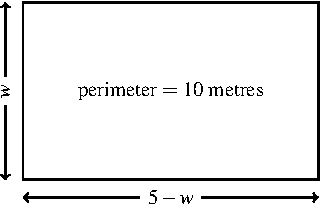
\includegraphics[scale=1]{image/09/largest-area.pdf}
\caption{%%
  A rectangle whose perimeter is ten metres.  The width is denoted as
  $w$ and the length is $5 - w$.
}
\label{fig:largest_area_rectangle}
\end{figure}

\begin{figure}[!htbp]
\centering
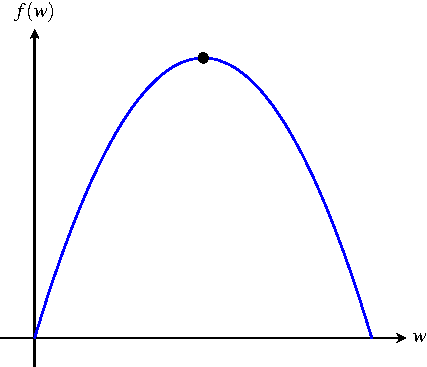
\includegraphics[scale=1]{image/09/rectangle-area.pdf}
\caption{%%
  The area $f(w) = (5 - w) w$ of a rectangle as a function of its
  width $w$.  The tip of the parabola is the highest point in the
  graph of $f(w)$.  Here, the tip point is also the point at which the
  value of $f(w)$, or the area, is largest.
}
\label{fig:largest_area_graph_parabola}
\end{figure}

\solutionpart{subex:largest_area_of_rectangle}
\Figure{fig:largest_area_graph_parabola} shows a graph of the function
$f(w)$.  Note the highest point in the graph.  The horizontal
coordinate~(i.e.~the value of $w$) gives you the width of the
rectangle.  The vertical coordinate~(i.e.~the value of $f(w)$) gives
you the corresponding area of the rectangle.  So the largest area of
the rectangle must occur at the tip point in the graph of $f(w)$.  You
know that \Equation{eqn:parabola_tip_x_coordinate} gives the
horizontal coordinate of the tip point of a quadratic function.  Using
\Equation{eqn:parabola_tip_x_coordinate} results in the horizontal
coordinate
%%
\begin{align*}
w
&=
-\frac{5}{2(-1)} \\[4pt]
&=
\frac{-5}{-2} \\[4pt]
&=
\frac{5}{2}
\end{align*}
%%
for the highest point of $f(w)$.  That is, the largest value of the
function $f(w)$ occurs when the width is $w = 5 / 2 = 2.5$ metres.
What about the actual value of $f(w)$?  Substitute $w = 5 / 2$ into
$f(w)$ to get
%%
\begin{align*}
f(5/2)
&=
\parenthesis*{5 - \frac{5}{2}} \frac{5}{2} \\[4pt]
&=
\parenthesis*{\frac{10}{2} - \frac{5}{2}} \frac{5}{2} \\[4pt]
&=
\frac{5}{2} \times \frac{5}{2} \\[4pt]
&=
\frac{25}{4}.
\end{align*}
%%
This tells you that the largest area the rectangle can have is
$25 / 4 = 6.25$ metres squared.
\end{solution}


%%%%%%%%%%%%%%%%%%%%%%%%%%%%%%%%%%%%%%%%%%%%%%%%%%%%%%%%%%%%%%%%%%%%%%%%%%%

\subsection*{Free fall}

You throw a ball straight up into the air.  The ball travels upward
for some time, reaches a maximum height, and then falls to the
ground.  Other than throwing the ball upward, you do not interfere
with the movement of the ball, but allow the forces of gravity and air
drag~(air resistance) to act on the ball.  In many cases, the force of
air drag can be ignored.  For now you only need to take into account
the force of gravity.  When the ball is allowed to move upward and
downward freely as described above, the motion of the ball is an
example of \emph{free fall}.

The position of the ball changes with time.  But precisely in what
way?  To analyse the position of the ball, let's make various
assumptions.  Denote by $t$ the time in seconds and let $f(t)$ be the
height in metres of the ball.  The \emph{initial height} of the ball
is the ball's height above ground level before the ball moves upward.
When you hold the ball in your hand just before you throw it upward,
the initial height of the ball is the distance~(in metres) from your
hand to the ground.  If the ball is on the ground before it moves
upward, its initial height is zero metres.  Let $h$ be the initial
height of the ball.  The \emph{initial velocity} of the ball is the
speed in metres per second with which the ball is thrown upward.
Denote the initial velocity of the ball by $v$.  The force of gravity
acts on the ball in a downward manner.  This is because gravity tends
to pull an object downward towards the centre of the Earth.  The force
of gravity is usually written as $g$ and its value is the constant of
$9.8$ metres per second squared.  To analyse the position of the ball,
you must take into account the initial height of the ball, the upward
distance it travels as time passes, and the downward force of gravity.
The position of the ball above ground level can be approximated by the
quadratic function
%%
\begin{equation}
\label{eqn:position_of_object_under_free_fall}
f(t)
=
-\frac{1}{2} gt^2 + vt + h.
\end{equation}

\begin{example}
\label{ex:spring_ball}
\textbf{Boing boing.}
A spring is located at ground level and can shoot a ball upward at an
initial velocity of $10$ metres per second.
%%
\begin{packedenum}
\item\label{ex:spring_ball_graph}
  Write down a function for the position of the ball and graph the
  function.

\item\label{ex:spring_ball_time_to_maximum_height}
  Determine the amount of time~(in seconds) required for the ball to
  reach maximum height.  Calculate the maximum height~(in metres) that
  the ball reaches.

\item\label{ex:spring_ball_time_hit_ground}
  When will the ball reach the ground?
\end{packedenum}
\end{example}

\begin{solution}
\solutionpart{ex:spring_ball_graph}
You know that the force of gravity is $g = 9.8$ metres per second
squared.  The initial velocity is $v = 10$ metres per second.  Since
the spring is located at ground level, let's assume that the initial
height of the ball is $h = 0$ metres.  Substitute these values into
\Equation{eqn:position_of_object_under_free_fall} and simplify the
result to get $f(t) = -\frac{49}{10}t^2 + 10t$, whose graph is shown
in \Figure{fig:spring_ball_graph}.  This is a rough sketch that
illustrates three points on which you should concentrate.  First is
the point at the origin $\tuple{0}{0}$ that tells you the initial
height of the ball at time $t = 0$ before the ball is shot upward.
Next is the tip point, which in this example is the highest point
$\tuple{a}{f(a)}$ of the graph of $f(t)$.  The tip point
$\tuple{a}{f(a)}$ tells you that the ball reaches its maximum height
of $f(a)$ metres above the ground at time $t = a$ seconds after being
shot upward by the spring.  The third point $\tuple{b}{0}$ tells you
approximately how long the ball is in the air before it lands on the
ground.  You do not yet know the values of $a$ and $b$.  This is just
a rough sketch to help you understand the example.

\begin{figure}[!htbp]
\centering
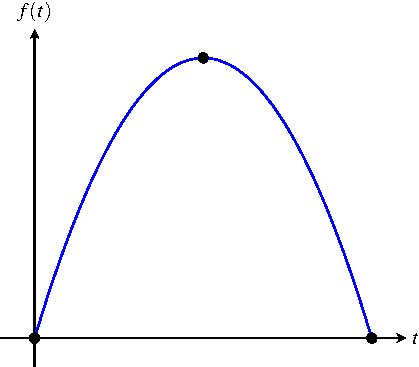
\includegraphics[scale=1]{image/09/spring-ball.pdf}
\caption{%%
  The height of a ball as a function of time.  Here, time $t$ is
  measured in seconds and the height $f(t)$ of the ball is measured in
  metres above the ground.
}
\label{fig:spring_ball_graph}
\end{figure}

\solutionpart{ex:spring_ball_time_to_maximum_height}
From \Formula{eqn:parabola_tip_x_coordinate} you know that the tip
point~(i.e. highest point) of the graph of $f(t)$ occurs at
$t = 50/49$.  This means that the ball reaches its maximum height
above the ground at approximately $t = 50/49 \approx 1.0204$
seconds~(rounded to four decimal places) after being shot up by the
spring.  The maximum height that the ball reaches is
$f(50 / 49) = 250 / 49$, which is approximately $5.1020$ metres above
the ground, rounded to four decimal places.

\solutionpart{ex:spring_ball_time_hit_ground}
You can use the quadratic formula to calculate the time at which the
ball hits the ground.  However, the following is a simple method that
does not use the quadratic formula.  Note that the function $f(t)$ can
be factorised as
%%
\begin{align*}
f(t)
&=
-\frac{49}{10} t^2 + 10t \\[4pt]
&=
\parenthesis*{-\frac{49}{10} t + 10} t \\[4pt]
&=
\parenthesis*{10 - \frac{49}{10} t} t.
\end{align*}
%%
Since the roots of $f(t)$ are those values of $t$ such that the
equation $f(t) = 0$ is true, this is the same as determining the
values of $t$ such that the following equation is true:
%%
\begin{equation}
\label{eqn:spring_ball_equation_factored}
\parenthesis*{10 - \frac{49}{10} t} t
=
0.
\end{equation}
%%
Equation~\eqref{eqn:spring_ball_equation_factored} is true when
$t = 0$.  However, the point $\tuple{0}{0}$ is the starting position
of the ball when it is initially on the ground.  So you can ignore the
root $t = 0$ of $f(t)$.  If the factor $10 - \frac{49}{10} t = 0$,
then \Equation{eqn:spring_ball_equation_factored} will also be true.
You must solve the equation $10 - \frac{49}{10} t = 0$ for $t$.  Doing
so gives you the root $t = 100 / 49$.  Therefore the ball will reach
the ground at approximately $t = 100 / 49 \approx 2.0408$ seconds
after being shot up by the spring.
\end{solution}

\begin{exercise}
You will verify the solution of \Example{ex:spring_ball}.
%%
\begin{packedenum}
\item\label{subex:spring_ball_height_function}
  Show that the height of the ball can be written as
  $f(t) = -\frac{49}{10} t^2 + 10t$.

\item\label{subex:spring_ball_highest_point}
  Show that the ball reaches its highest point at $t = 50 / 49$
  seconds after being shot up.  Also show that the highest point is
  $f(50 / 49) = 250 / 49$ metres above the ground.

\item\label{subex:spring_ball_quadratic_formula}
  Use the quadratic formula to calculate the roots of $f(t)$.
\end{packedenum}
\end{exercise}
%%
\ifbool{showSolution}{
\begin{solution}
\solutionpart{subex:spring_ball_height_function}
You have the values $g = 9.8 = 49/5$, $v = 10$, and $h = 0$.
Substitute these values into
\Equation{eqn:position_of_object_under_free_fall} to obtain
%%
\begin{align*}
f(t)
&=
-\frac{49}{5} \times \frac{1}{2} t^2 + 10t + 0 \\[4pt]
&=
-\frac{49}{10} t^2 + 10t.
\end{align*}

\solutionpart{subex:spring_ball_highest_point}
Use \Expression{eqn:parabola_tip_x_coordinate} to get
%%
\begin{align*}
t
&=
-\frac{10}{2 \times \parenthesis*{-\frac{49}{10}}} \\[4pt]
&=
\frac{10}{\frac{49}{5}} \\[4pt]
&=
10 \times \frac{5}{49} \\[4pt]
&=
\frac{50}{49}.
\end{align*}
%%
Then you have the function value
%%
\begin{align*}
f(50 / 49)
&=
-\frac{49}{10} \parenthesis*{\frac{50}{49}}^2
+
10\parenthesis*{\frac{50}{49}} \\[4pt]
&=
-\frac{49}{10} \times \frac{50^2}{49^2}
+
\frac{10 \times 50}{49} \\[4pt]
&=
-\frac{5 \times 50}{49}
+
\frac{10 \times 50}{49} \\[4pt]
&=
\frac{
  50(10 - 5)
}{
  49
} \\[4pt]
&=
\frac{
  250
}{
  49
}.
\end{align*}
%%

\solutionpart{subex:spring_ball_quadratic_formula}
Using the quadratic formula results in
%%
\begin{align*}
t
&=
\frac{
  -(10) \pm \sqrt{10^2 - 4\parenthesis*{-\frac{49}{10}} (0)}
}{
  2 \parenthesis*{-\frac{49}{10}}
} \\[4pt]
&=
\frac{
  -10 \pm \sqrt{10^2}
}{
  -\frac{49}{5}
} \\[4pt]
&=
\frac{
  -10 \pm 10
}{
  -\frac{49}{5}
}.
\end{align*}
%%
The roots of $f(t)$ are
\[
t_1
=
\frac{
  -10 + 10
}{
  -\frac{49}{5}
}
=
0
%%
\qquad
\text{and}
\qquad
%%
t_2
=
\frac{
  -10 - 10
}{
  -\frac{49}{5}
}
=
\frac{100}{49}.
\]

\end{solution}
}{}

\end{document}
